\lecture{7}{Tue 13 Sep 2022 12:02}{}

$f'(z) = m(z-a)^{m-1 }g(z) + (z-a)^mm g'(z)$ 
Rule: a zero of multiplicity $m$ if \[
	f(a) = f'(a) = \ldots = f^{(m-1)}(a) = 0
.\] 
but $f^{(m)}(a) \neq  0$

\subsection{Partial Fractions Decomposition}

For any $\frac{p}{q}$, if $\operatorname{deg} p \ge \operatorname{deg} q$, we can divide with remainder to obtain \[
	\frac{p}{q} = g + \frac{r}{q}, \operatorname{deg} r < \operatorname{deg} q
.\] 
In other words, $\frac{r}{q}(\infty ) = 0$. Such rational functions are \textit{proper}.

Now we decompose the proper rational functions to sum of \textit{simple} fractions.

\[
	\frac{p}{q} = g + \sum_{j=1}^{k} \sum_{i =1}^{mj } \frac{c_{j i}}{\left( z - a_j \right) ^i}
.\] 
We could treat  $c_{ji }$ as \textit{undetermined coefficients}, and obtain a linear system of equations. There's a simpler way to get the coefficients, though.

\begin{example}
	\begin{enumerate}
		\item 
	\[
		\frac{1}{z\left( z-1 \right) (z-2)} = \frac{A}{z}+\frac{B}{z-1}+\frac{C}{z-2}
	.\] 

	To find $A$, multiply by $z$, and plug $z = 0$.
	\[
		\frac{1}{(z-1)(z-2)} = A \implies A = \frac{1}{(-1)(-2) }= \frac{1}{2}
	.\] 
	Similarly $B = -1$ and $C = \frac{1}{2}$.
\item \[
	\frac{z^3}{z^2 - 1} = z + \frac{z}{(z-1)(z+1)} = z + \frac{A}{z-1}+\frac{B}{z+1}
.\] 
\item \[
	\frac{z}{z^2 + 1} = \frac{A}{z-i} + \frac{B}{z+i}
.\] 
We have $A = B = \frac{1}{2}$
\item \[
	\frac{z}{(z+i)^2} = \frac{A}{z+i} + \frac{B}{(z+i)^2}
.\] 
pole at $-1$, with multiplicity $2$.

To find $B$, multiply by $(z+i)^2$ and plug  $z=-i$. To find $A$, multiply by $(z+i)^2$, differentiate, and plug $z = -i$.
\[
	A = \frac{d}{dz}(z) |_{z = -i} = 1
.\] 
	\end{enumerate}
\end{example}

Now we find the general formula.
\[
	c_{j,k} = \frac{1}{(k-1)!}\frac{d^{(k-1)}}{dz^{k-1}} \left. \left( (z-a_j)^{mj }f(z) \right) \right|_{z = a_j}
.\] 

\subsection{Trigonometric, Hyperbolic and Logarithmics Function}

$e^z$, $\cos z = \frac{1}{2}(e^{iz} + e^{-iz })$, $\sin z = \frac{1}{2i } \left( e^{iz }- e^{-iz } \right) $ are entire.

 $\tan z = \frac{\sin z}{\cos z}$, poles where $\cos z = 0$ 

\begin{example}
	$\cos iz = \frac{1}{2}(e^{-z} + e^z) =: \text{ch} z (\cosh z)$ 

	$\sin iz = \frac{i}{2}(e^{-z} - e^z) =:i \text{sh} z (\sinh z)$ 

	$\cos z = \frac{1}{2} (e^y + e^{-y}) \cos x - i \frac{1}{2} (e^y - e^{-y}) \sin x = \text{ch} y \cos x - i \text{sh} y \sin x$

\end{example}

$e^z = w$ (no solutions when $w = 0$, infinitely many solution for $w \neq  0$ )

$e^{x+iy } = |w| e^{i \operatorname{arg} w}$, $\varphi = \operatorname{arg}  w $ (infinitely many)

$e^x = |w|$, $x = \operatorname{Log} w$ (real number, "high school" log)

$y = \operatorname{arg} w = \operatorname{Arg} w + 2 \pi k, k \in \mathbb{Z}$, 

$\operatorname{Arg} w = (-\pi, \pi] \cap  \operatorname{arg} w$ (single number)

\begin{remark}
	 Main disadvantage of $\operatorname{Arg}$ is its \textbf{dis-continuity} at $-\pi$. We need functions to be continuous in order to plug values into them.

	 We may even make $Arg w \in (-\pi, \pi)$ to avoid dealing with the nagetive real line. We have made a branch cut.
\end{remark}

Now we want to define $\log$ such that $z = \log w$ contains all solutions, infinity many of them.

\begin{align*}
	z &= \log w \\
	&= \operatorname{Log} |w| + i \operatorname{Arg} w + 2 \pi i k,\qquad k \in \mathbb{Z}\\
	\operatorname{Log} w &:= \operatorname{Log} |w| + i \operatorname{Arg}  w
.\end{align*}

$\operatorname{Log} w $ is the  \textit{principal branch} of the $\log$.


\begin{example}
	Solve $\cos z = 2$.
	
	If want to solve $f(g(z)) = w$, first solve for $g(z)$, and then solve for $z$.

	\[
		\cos z = \frac{1}{2} (e^{iz} + e^{-iz}) = J\left( e^{i z} \right)
	.\] 
	\begin{enumerate}
		\item Let $\zeta = e^{iz}$ and we now solve $J(\zeta) = 2$, which is a quadratic.
	\begin{align*}
		\zeta^2 + 4 \zeta + 1 &= 0\\
		\zeta = 2 \pm \sqrt{3} 
	.\end{align*} 

\item Solve $e^{iz } = \zeta$.
	\begin{align*}
		e^{i z = 2 + \sqrt{3} } \implies i z_{1,k} &= Log \zeta_1 + 2 \pi i k, \quad k \in \mathbb{Z}\\
 z_{1,k} &= - i Log \left( 2 + \sqrt{ 3}  \right)  + 2 \pi k, \quad k \in \mathbb{Z}\\
 e^{i z = 2 - \sqrt{3} } \implies i z_{2,k} &= Log \left( 2 - \sqrt{3}  \right)  + 2 \pi i k, \quad k \in \mathbb{Z}\\
 z_{2, k} &= - i Log(2 - \sqrt{3} ) + 2 \pi k
	.\end{align*}
	Now we make a picture of the solutions.
	\end{enumerate}
	Since $\zeta_1 \zeta_2 = 1$, $\operatorname{Log} \zeta_1 = - \operatorname{Log} \zeta_2 $. So the solutions are in pairs symmetric by the $x$ axis.

	How does the solution to $\cos z = t$ evolve when $t $ changes? See visualization:
		
\end{example}

\subsubsection{Logarithmic and Exponential}


\begin{figure}[H]
	\centering
	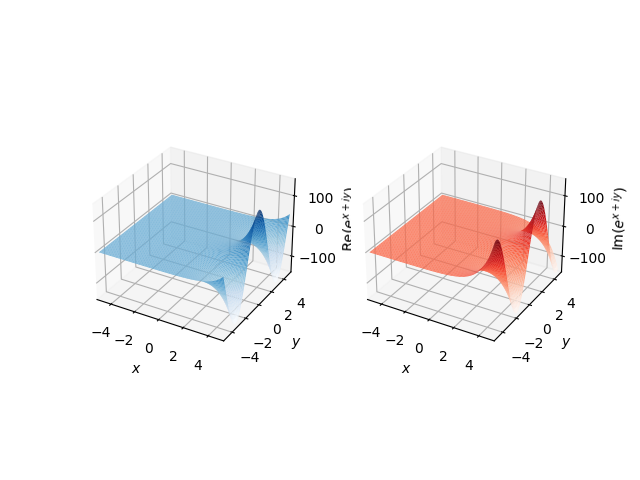
\includegraphics[width=0.8\textwidth]{figures/exp_z.png}
	\caption{$\exp(x+i y)$}
	\label{fig:exp_z}
\end{figure}
\textbf{Properties of }$\exp(z)$ 
\begin{enumerate}
	\item \textbf{Definition:}
	\item \textbf{Domain/Range:} 
	\item \textbf{Derivative/Antiderivative:} 
	\item \textbf{Branch cut:} 
\end{enumerate}

\begin{figure}[H]
	\centering
	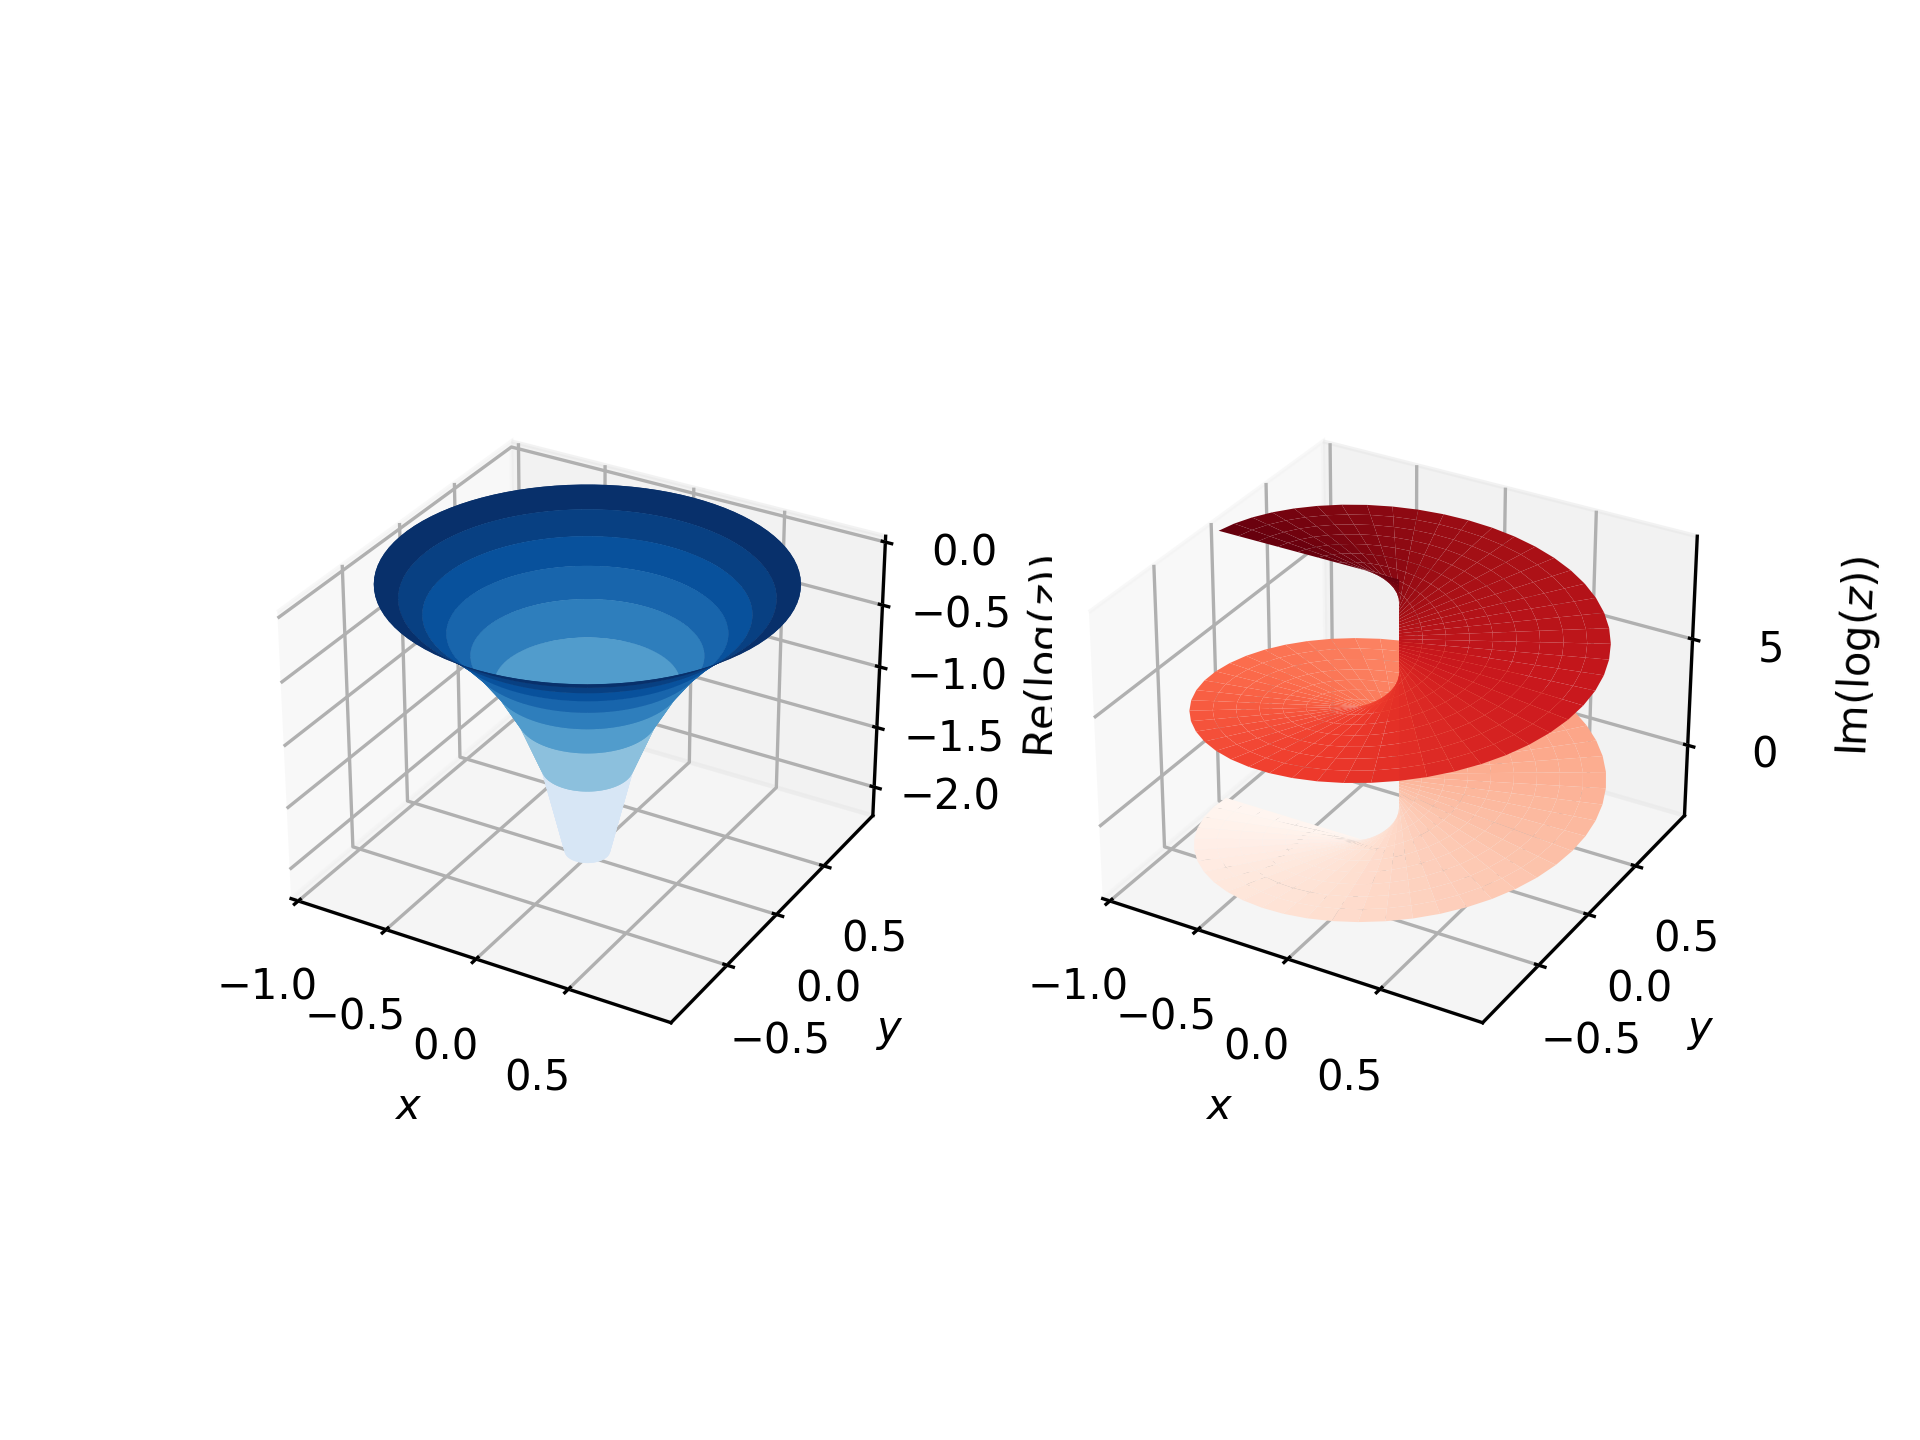
\includegraphics[width=0.8\textwidth]{figures/log_z.png}
	\caption{$\log(x+i y)$}
	\label{fig:log_z}
\end{figure}
\textbf{Properties of }$\log(z)$ 

\begin{enumerate}
	\item \textbf{Definition:} If $z \neq 0$, then we define $\log z$ to be the set of infinitely many values
\[
\begin{aligned}
\log z: &=\log |z|+i \arg z \\
&=\log |z|+i \operatorname{Arg} z+i 2 k \pi \quad(k=0, \pm 1, \pm 2, \ldots)
\end{aligned}
\]
	\item \textbf{Domain/Range:} 
		\begin{theorem}
		The function $\log z$ is analytic in the domain $D^*$ consisting of all points of the complex plane except those lying on the nonpositive real axis (see Fig. 3.3). Furthermore,
\[
\frac{d}{d z} \log z=\frac{1}{z}, \quad \text { for } z \text { in } D^*
\]
		\end{theorem}	
		\begin{corollary}
			The function $\operatorname{Arg} z$ is harmonic in the domain $D^*$ of the previous theorem.
		\end{corollary}
		\begin{corollary}
			The real function $\log |z|$ is harmonic in the entire plane with the exception of the origin.
		\end{corollary}
	\item \textbf{Derivative/Antiderivative:} 
		$\begin{aligned} \frac{d}{d z} \log _b z &=\frac{1}{z \ln b} \\ \int \log _b z d z &=\frac{z(\ln z-1)}{\ln b}+C . \end{aligned}$
	\item \textbf{Branch cut:} $\log z:=\log |z|+i \operatorname{Arg} z$
	\item \textbf{Identities:}
\end{enumerate}
\subsubsection{Trigonometric Functions}
\begin{figure}[H]
	\centering
	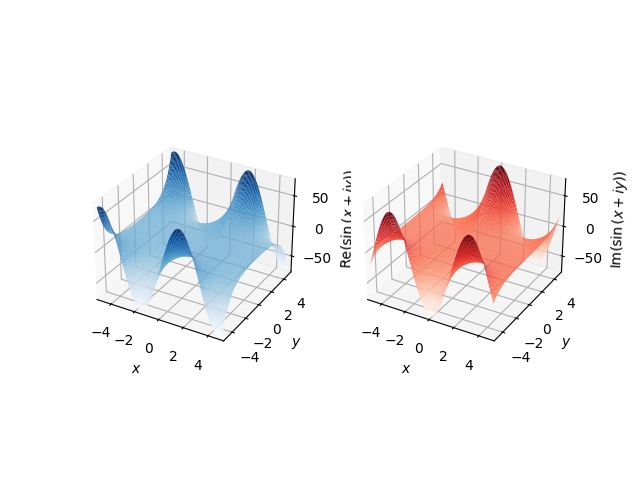
\includegraphics[width=0.8\textwidth]{figures/sin_z.png}
	\caption{$\sin(x+i y)$}
	\label{fig:sin_z}
\end{figure}
\textbf{Properties of }$\sin(z)$ 

\begin{enumerate}
	\item \textbf{Definition:} $\begin{aligned} \sin z &=\frac{e^{i z}-e^{-i z}}{2 i} \\ &=\frac{1}{2} i\left(e^{-i z}-e^{i z}\right) \end{aligned}$
		The sine function can be defined analytically by the infinite sum
\[
\sin x=\sum_{n=1}^{\infty} \frac{(-1)^{n-1}}{(2 n-1) !} x^{2 n-1} .
\]
It is also given by the imaginary part of the complex exponential
\[
\sin x=\mathbb{I}\left[e^{i x}\right] .
\]
The multiplicative inverse of the sine function is the cosecant, defined as
\[
\csc x \equiv \frac{1}{\sin x} .
\]
	\item \textbf{Domain/Range:} 
	\item \textbf{Derivative/Antiderivative:} 
		The derivative of $\sin x$ is
\[
\frac{d}{d x} \sin x=\cos x
\]
and its indefinite integral is
\[
\int \sin x d x=-\cos x+C,
\]
where $C$ is a constant of integration.
	\item \textbf{Branch cut:} 
	\item \textbf{Identities:}
\end{enumerate}

\begin{figure}[H]
	\centering
	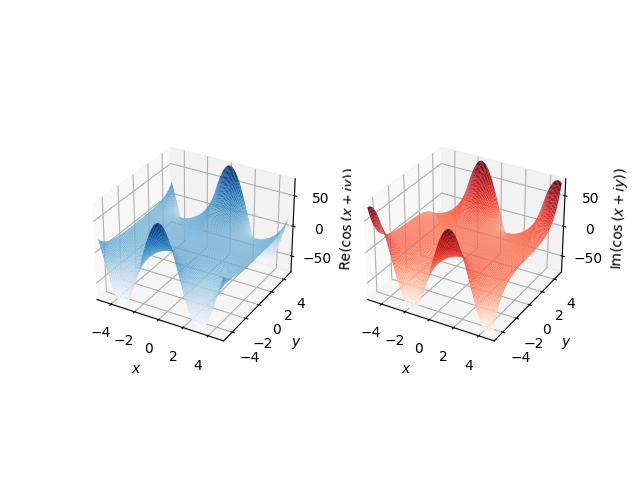
\includegraphics[width=0.8\textwidth]{figures/cos_z.png}
	\caption{$\cos(x+i y)$}
	\label{fig:cos_z}
\end{figure}
\textbf{Properties of }$\cos(z)$ 

\begin{enumerate}
	\item \textbf{Definition:}$\cos z=\frac{1}{2}\left(e^{i z}+e^{-i z}\right)$
		The cosine function can be defined analytically using the infinite sum
\[
\begin{aligned}
\cos x & \equiv \sum_{n=0}^{\infty} \frac{(-1)^n x^{2 n}}{(2 n) !} \\
&=1-\frac{x^2}{2 !}+\frac{x^4}{4 !}-\frac{x^6}{6 !}+\ldots,
\end{aligned}
\]
	\item \textbf{Domain/Range:} 
	\item \textbf{Derivative/Antiderivative:} 
	\item \textbf{Branch cut:} 
	\item \textbf{Identities:}
\end{enumerate}

\begin{figure}[H]
	\centering
	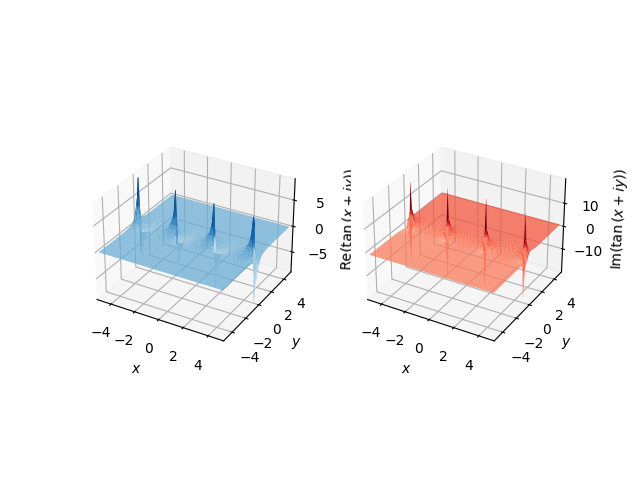
\includegraphics[width=0.8\textwidth]{figures/tan_z.png}
	\caption{$\tan(x+i y)$}
	\label{fig:tan_z}
\end{figure}
\textbf{Properties of }$\tan(z)$ 

\begin{enumerate}
	\item \textbf{Definition:} The definition of the tangent function can be extended to complex arguments $z$ using the definition
\[
\begin{aligned}
\tan z &=\frac{i\left(e^{-i z}-e^{i z}\right)}{e^{-i z}+e^{i z}} \\
&=\frac{e^{i z}-e^{-i z}}{i\left(e^{i z}+e^{-i z}\right)} \\
&=\frac{i\left(1-e^{2 i z}\right)}{1+e^{2 i z}} \\
&=\frac{e^{2 i z}-1}{i\left(e^{2 i z}+1\right)}
\end{aligned}
\]
	\item \textbf{Domain/Range:} 
	\item \textbf{Derivative/Antiderivative:} 
	\item \textbf{Branch cut:} 
	\item \textbf{Identities:}
		An important tangent identity is given by
\[
\tan ^2 \theta+1=\sec ^2 \theta
\]
Angle addition, subtraction, half-angle, and multiple-angle formulas are given by
\[
\begin{aligned}
\tan (\alpha+\beta) &=\frac{\tan \alpha+\tan \beta}{1-\tan \alpha \tan \beta} \\
\tan (\alpha-\beta) &=\frac{\tan \alpha-\tan \beta}{1+\tan \alpha \tan \beta} \\
\tan (2 \alpha) &=\frac{2 \tan \alpha}{1-\tan ^2 \alpha} \\
\tan (n \alpha) &=\frac{\tan [(n-1) \alpha]+\tan \alpha}{1-\tan [(n-1) \alpha] \tan \alpha} \\
\tan \left(\frac{\alpha}{2}\right) &=\frac{\sin \alpha}{1+\cos \alpha} \\
&=\frac{1-\cos \alpha}{\sin \alpha} \\
&=\frac{\tan \alpha \sin \alpha}{\tan \alpha+\sin \alpha}
\end{aligned}
\]
The sine and cosine functions can conveniently be expressed in terms of a tangent as
\[
\cos t=\frac{1-\tan ^2\left(\frac{1}{2} t\right)}{1+\tan ^2\left(\frac{1}{2} t\right)}
\]
\[
\sin t=\frac{2 \tan \left(\frac{1}{2} t\right)}{1+\tan ^2\left(\frac{1}{2} t\right)}
\]
\end{enumerate}


\subsubsection{Inverse Trigonometric Functions}

\begin{figure}[H]
	\centering
	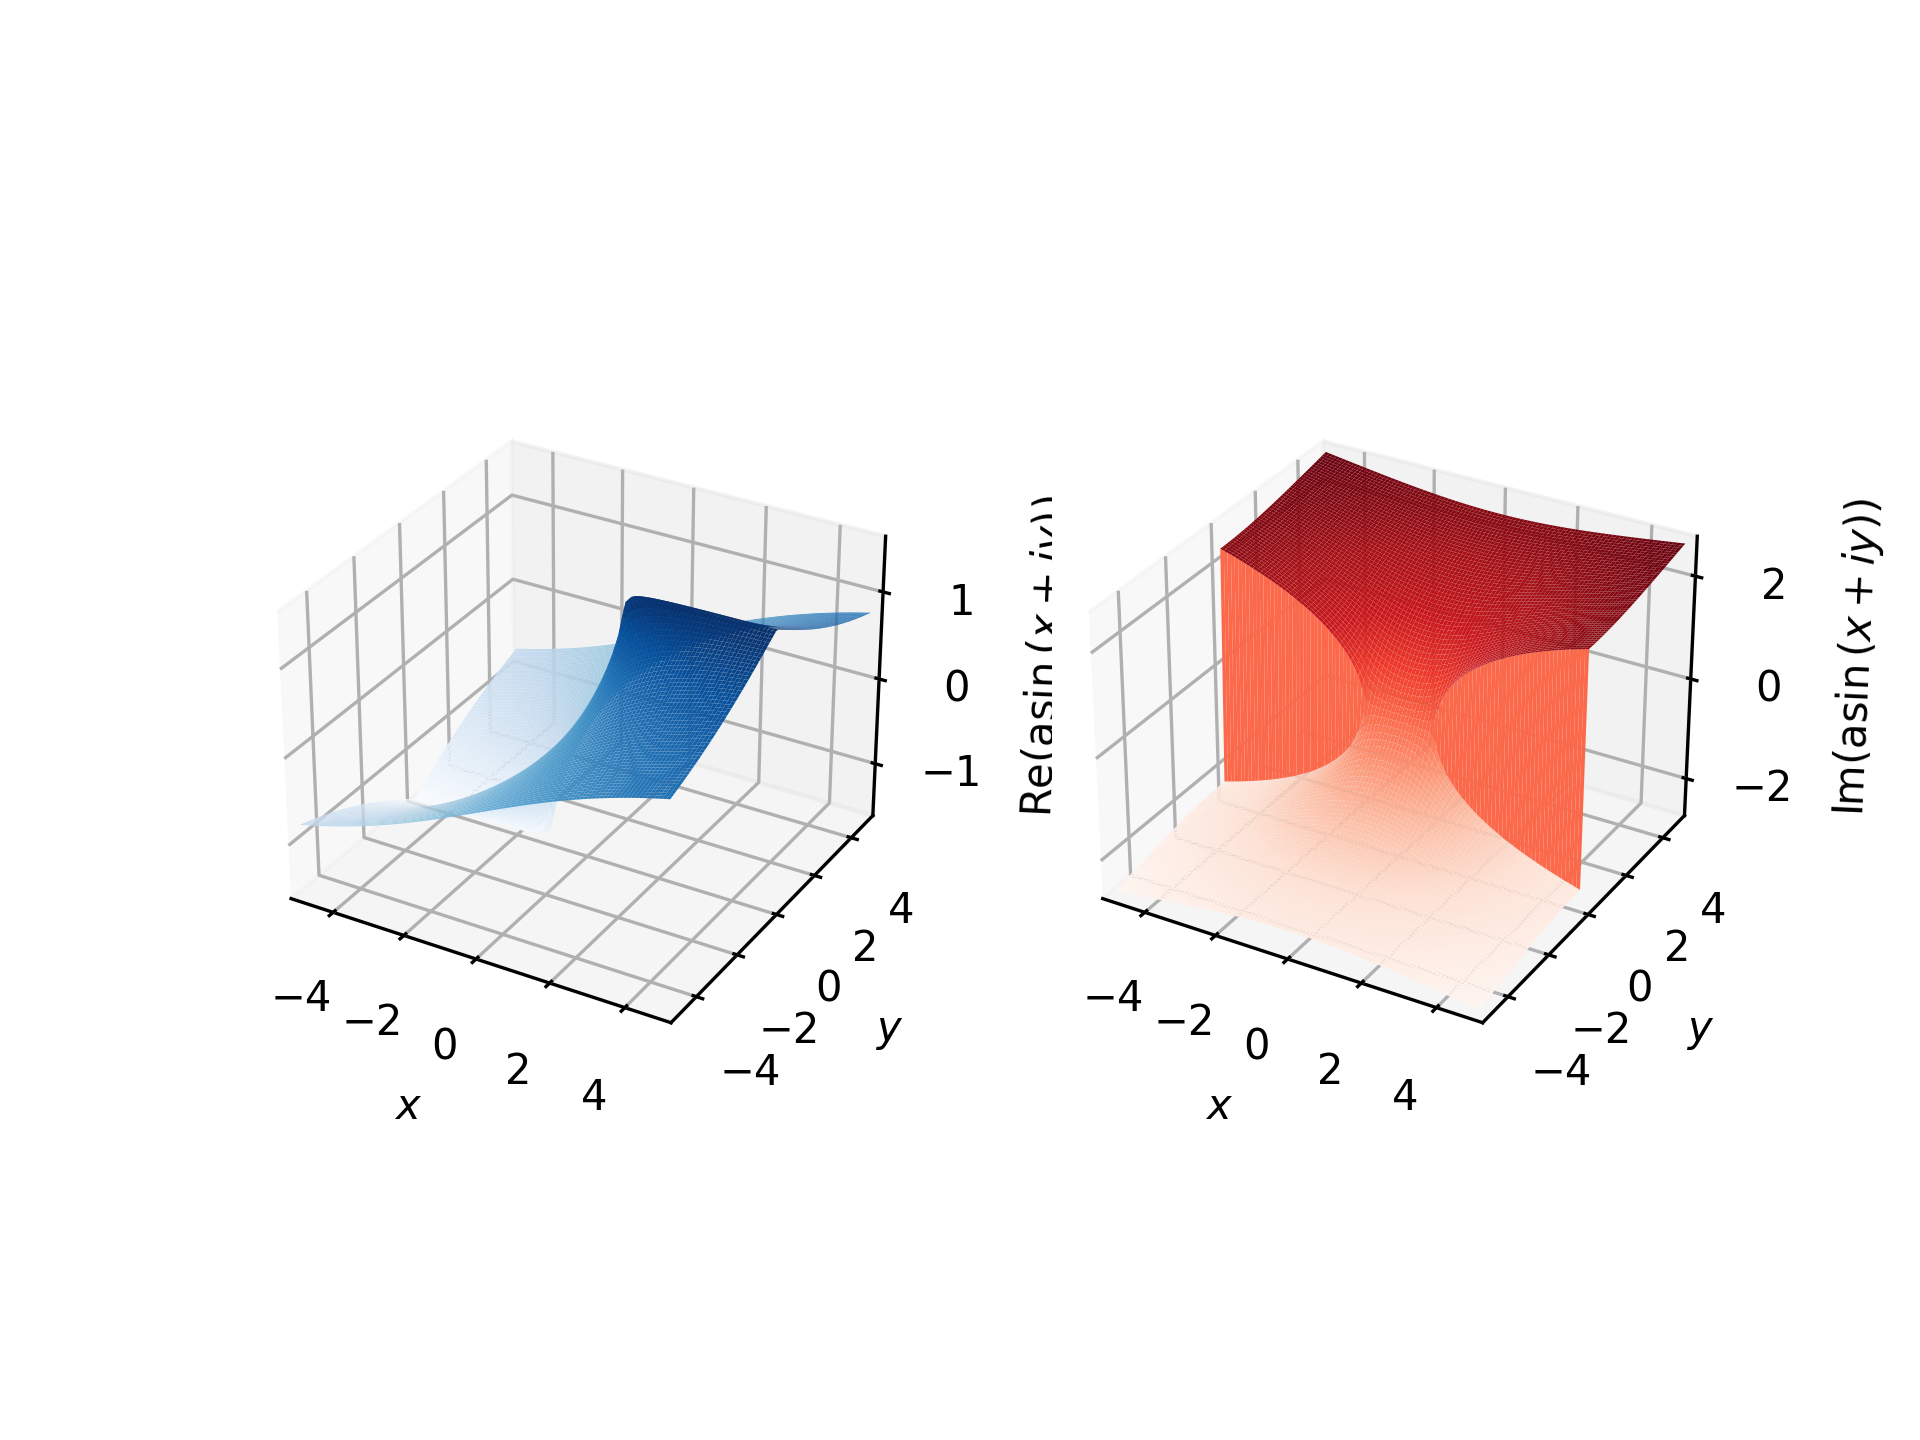
\includegraphics[width=0.8\textwidth]{figures/asin_z.png}
	\caption{$\arcsin(x+i y)$}
	\label{fig:arcsin_z}
\end{figure}
\textbf{Properties of }$\arcsin(z)$ 

\begin{enumerate}
	\item \textbf{Definition:} $\sin ^{-1} z=-i \ln \left(i z+\sqrt{1-z^2}\right)$
	\item \textbf{Domain/Range:} 
	\item \textbf{Derivative/Antiderivative:} 
		The derivative of $\sin ^{-1} z$ is
\[
\frac{d}{d z} \sin ^{-1} z=\frac{1}{\sqrt{1-z^2}}
\]
and its indefinite integral is
\[
\int \sin ^{-1} z d z=\sqrt{1-z^2}+z \sin ^{-1} z+C .
\]
	\item \textbf{Branch cut:} 
	\item \textbf{Identities:}
\end{enumerate}

\begin{figure}[H]
	\centering
	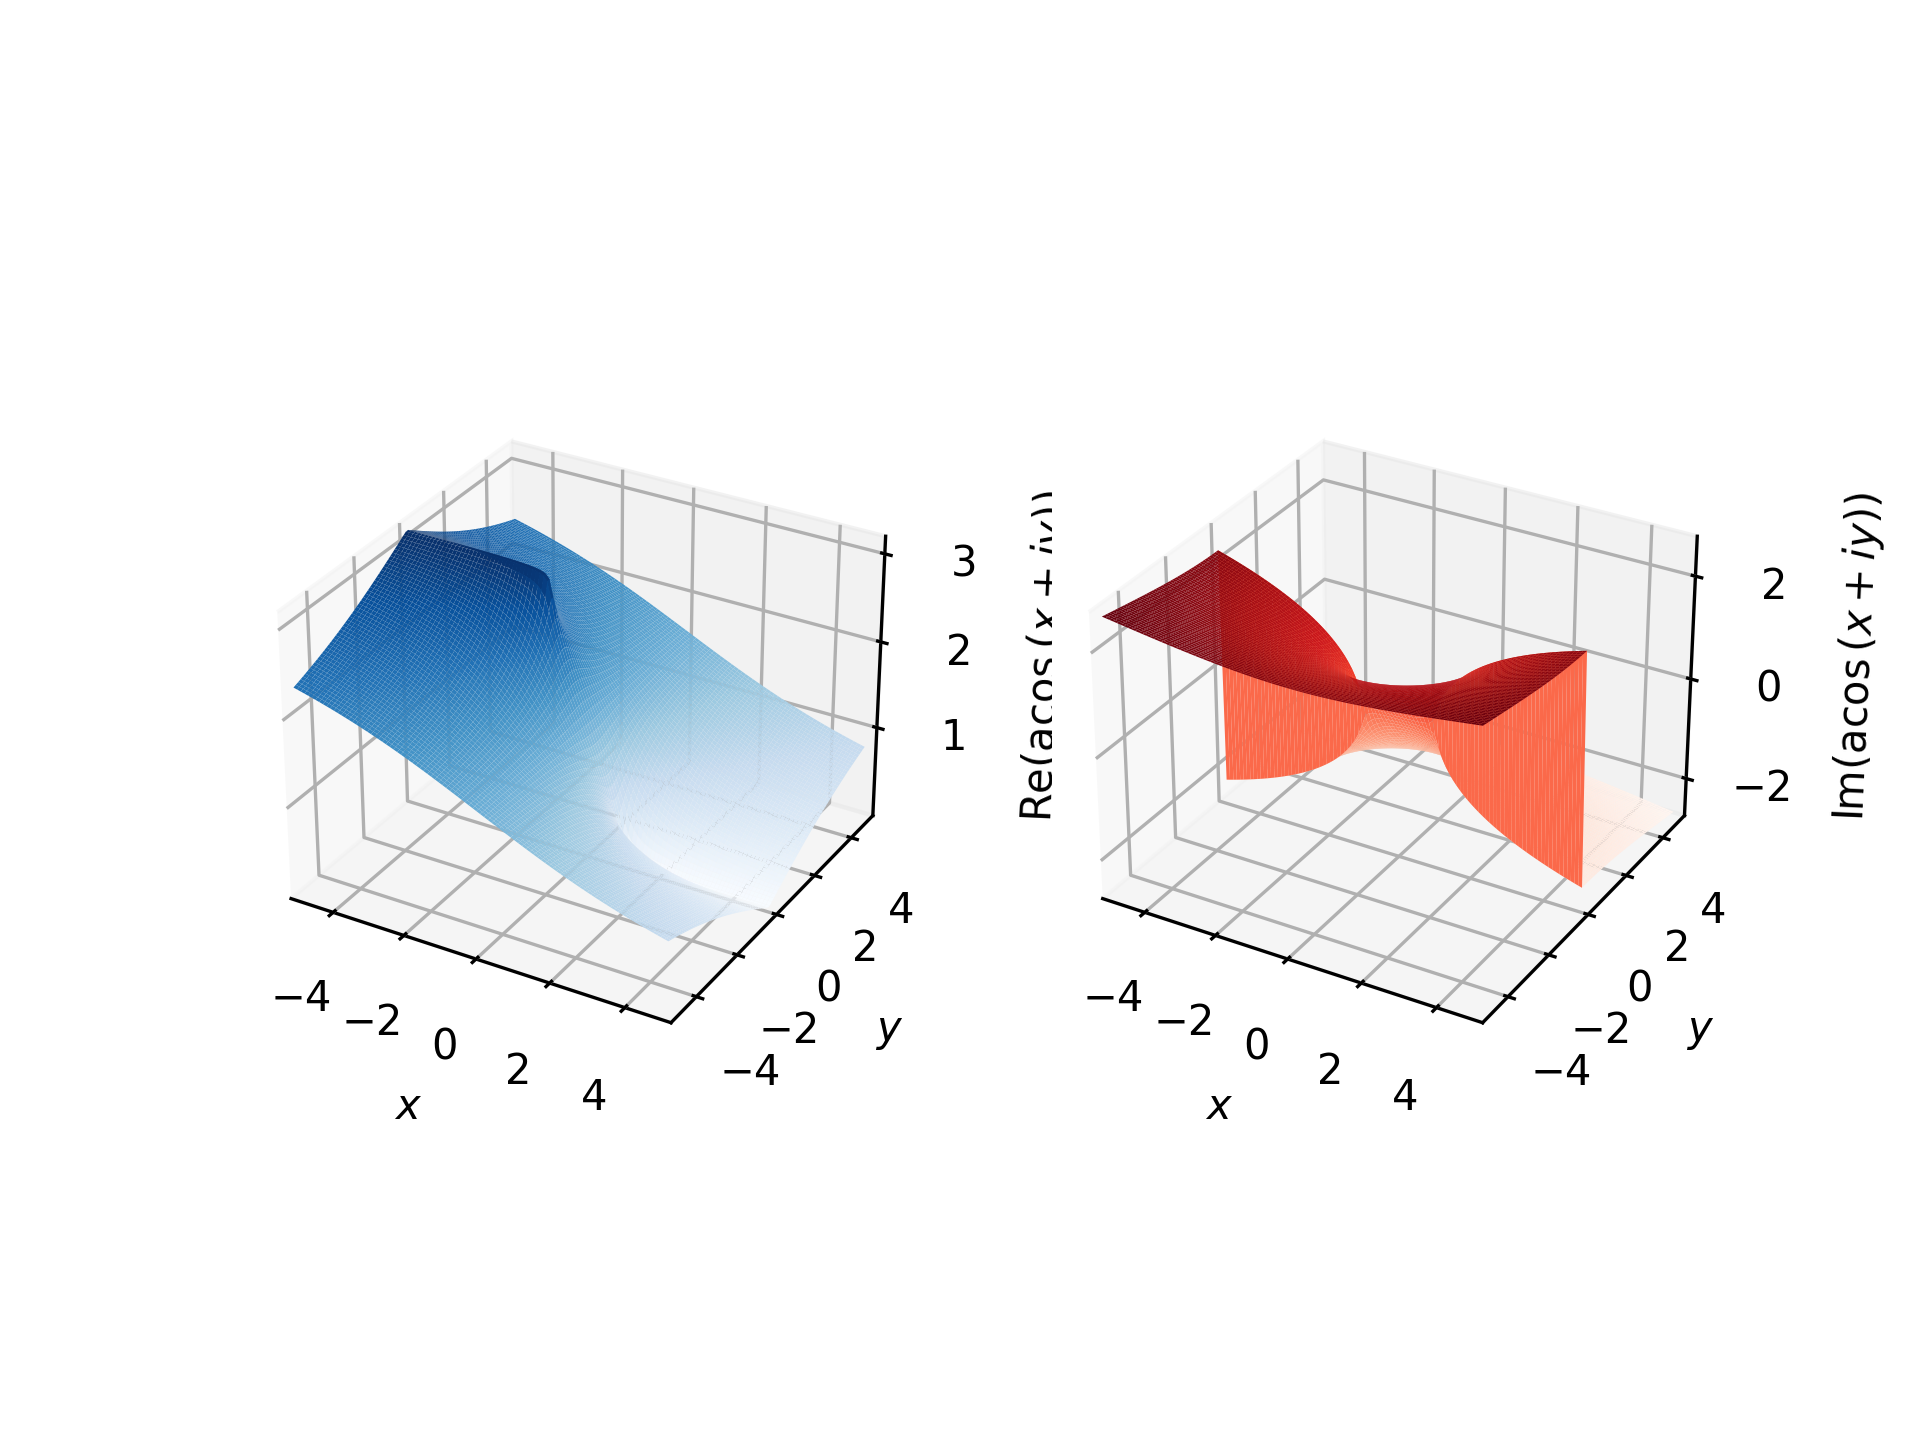
\includegraphics[width=0.8\textwidth]{figures/acos_z.png}
	\caption{$\arccos(x+i y)$}
	\label{fig:arccos_z}
\end{figure}
\textbf{Properties of }$\arccos(z)$ 

\begin{enumerate}
	\item \textbf{Definition:} $\cos ^{-1} z=\frac{1}{2} \pi+i \ln \left(i z+\sqrt{1-z^2}\right)$
	\item \textbf{Domain/Range:} 
	\item \textbf{Derivative/Antiderivative:} 
		The derivative of $\cos ^{-1} z$ is given by
\[
\frac{d}{d z} \cos ^{-1} z=-\frac{1}{\sqrt{1-z^2}}
\]
and its indefinite integral is
\[
\int \cos ^{-1} z d z=z \cos ^{-1} z-\sqrt{1-z^2}+C
\]
	\item \textbf{Branch cut:} 
	\item \textbf{Identities:}
		The inverse cosine satisfies
\[
\cos ^{-1} z=\pi-\cos ^{-1}(-z)
\]
for all complex $z$, and
\[
\cos ^{-1} x= \begin{cases}\frac{1}{2} \pi+\cos ^{-1}\left(\sqrt{1-x^2}\right) & \text { for } x \leq 0 \\ \frac{1}{2} \pi-\cos ^{-1}\left(\sqrt{1-x^2}\right) & \text { for } x \geq 0\end{cases}
\]
The inverse cosine is given in terms of other inverse trigonometric functions by
\[
\begin{aligned}
\cos ^{-1} z &=\frac{1}{2} \pi+\sin ^{-1}(-z) \\
&=\frac{1}{2} \pi-\sin ^{-1} z
\end{aligned}
\]
for all complex $z$.
\end{enumerate}

\begin{figure}[H]
	\centering
	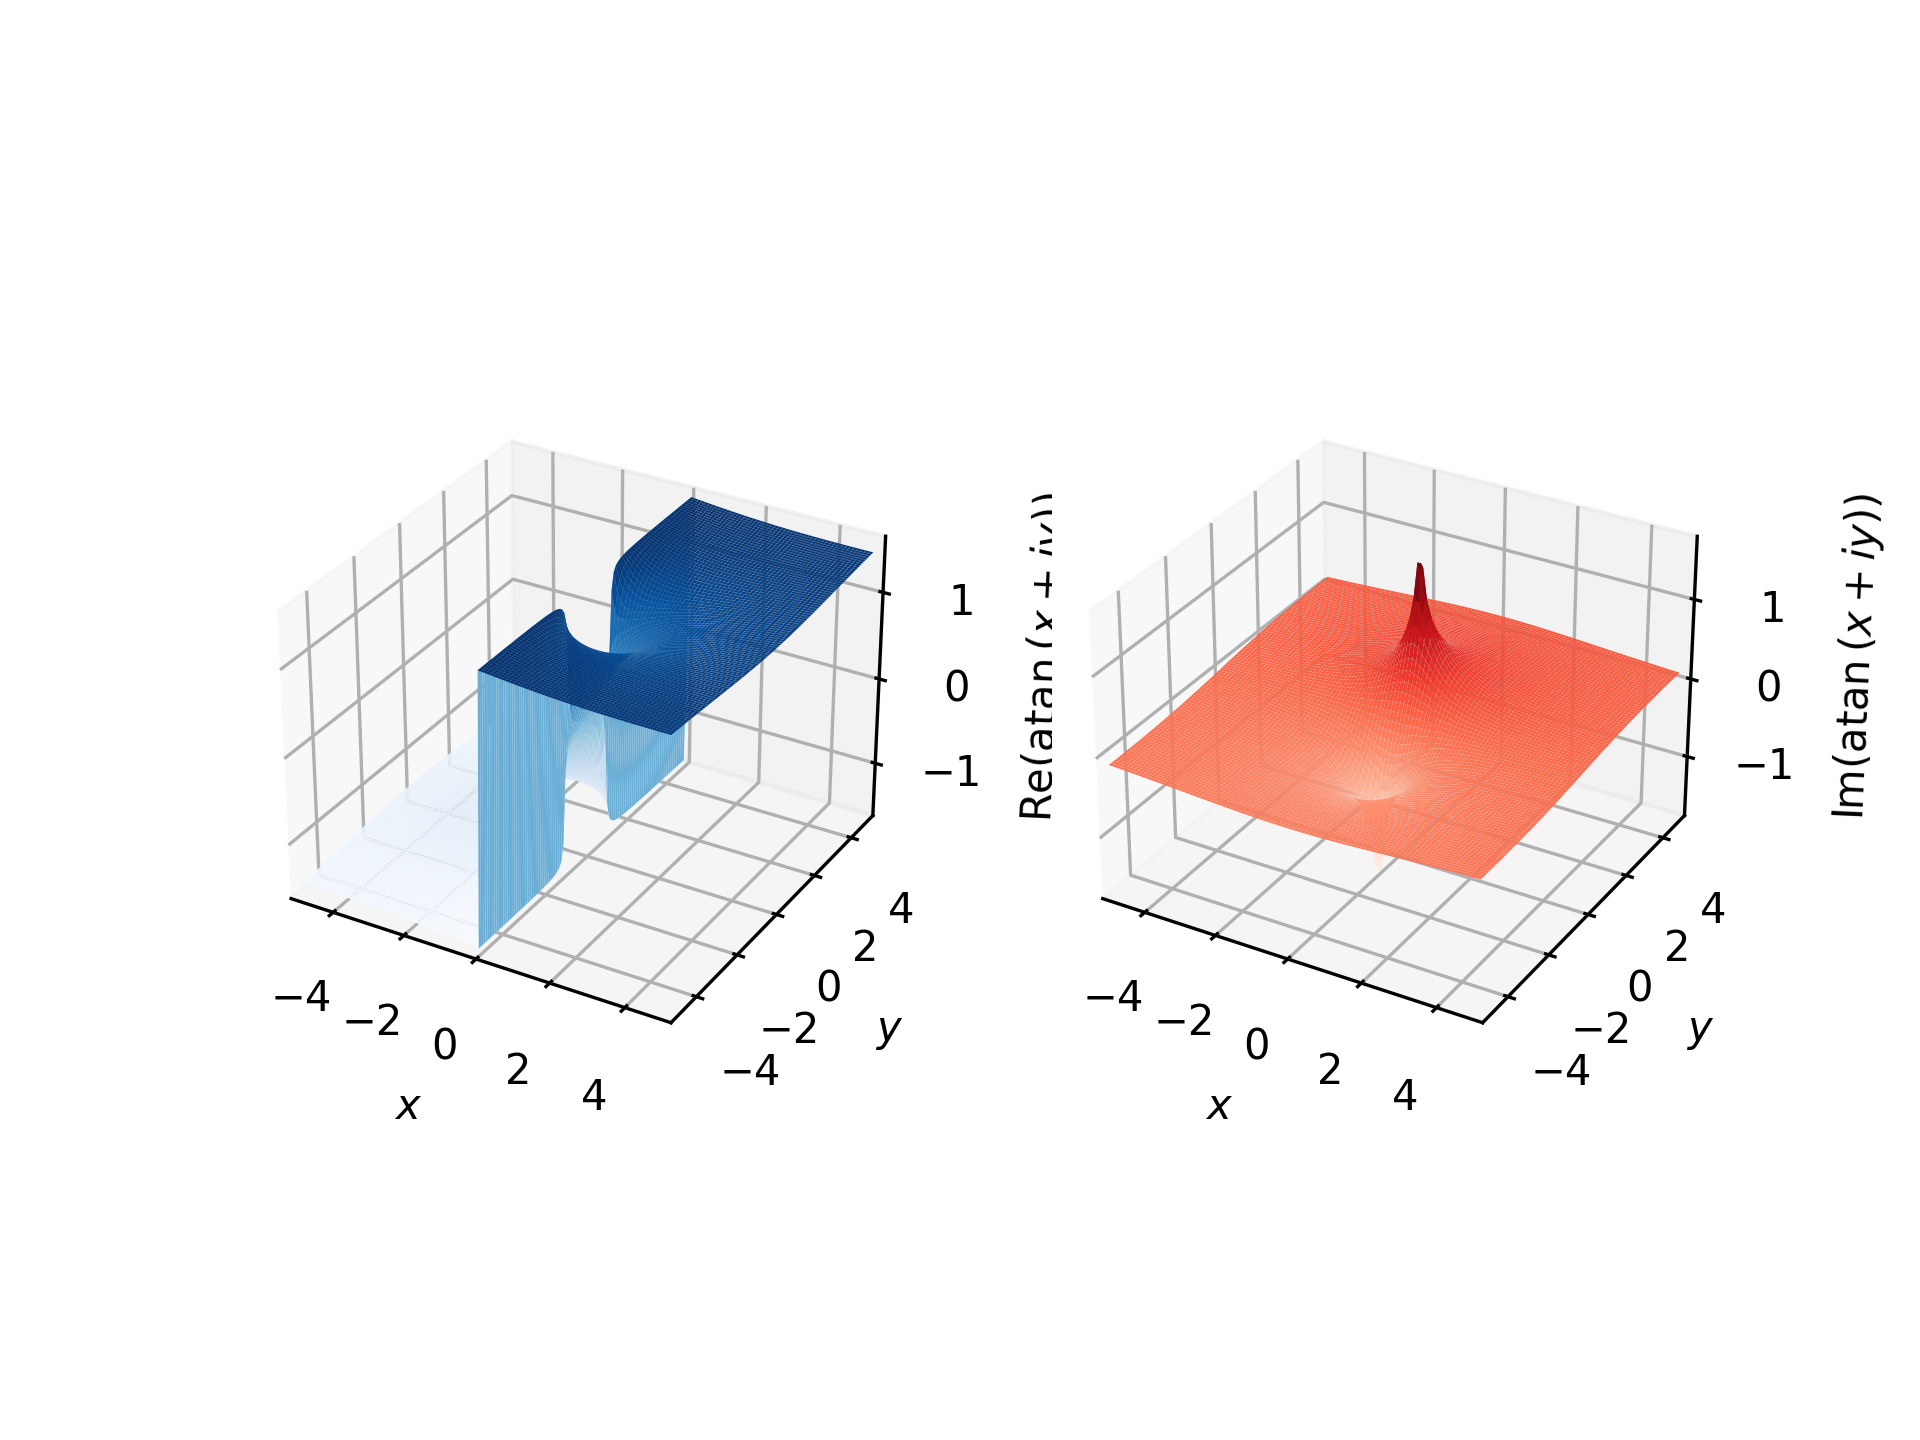
\includegraphics[width=0.8\textwidth]{figures/atan_z.png}
	\caption{$\arctan(x+i y)$}
	\label{fig:arctan_z}
\end{figure}
\textbf{Properties of }$\arctan(z)$ 

\begin{enumerate}
	\item \textbf{Definition:} $\tan ^{-1} z=\frac{1}{2} i[\ln (1-i z)-\ln (1+i z)]$
	\item \textbf{Domain/Range:} 
	\item \textbf{Derivative/Antiderivative:} The derivative of $\tan ^{-1} z$ is
\[
\frac{d}{d z} \tan ^{-1} z=\frac{1}{1+z^2}
\]
and the indefinite integral is
\[
\int \tan ^{-1} z d z=z \tan ^{-1} z-\frac{1}{2} \ln \left(1+z^2\right)+C .
\]
	\item \textbf{Branch cut:} 
	\item \textbf{Identities:}
The inverse tangent satisfies
\[
\tan ^{-1} z=\cot ^{-1}\left(\frac{1}{z}\right)
\]
for $z \neq 0$,
\[
\tan ^{-1} z=-\tan ^{-1}(-z)
\]
for all complex $z$,
\[
\begin{aligned}
\tan ^{-1} x &=\frac{1}{2} \pi-\cos ^{-1}\left(\frac{x}{\sqrt{x^2+1}}\right) \\
&=\sin ^{-1}\left(\frac{x}{\sqrt{x^2+1}}\right) \\
&=\csc ^{-1}\left(\frac{\sqrt{x^2+1}}{x}\right)
\end{aligned}
\]
for all real $x$, where equality for the last equation is understood to be in the limit as $x \rightarrow 0$.
\end{enumerate}


\subsubsection{Hyperbolic Functions}

\begin{figure}[H]
	\centering
	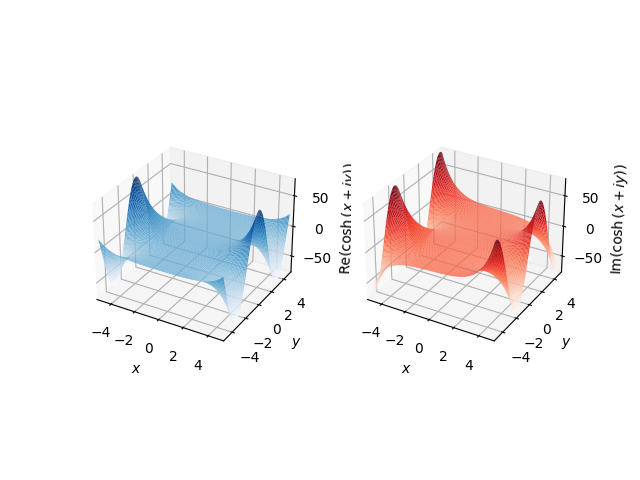
\includegraphics[width=0.8\textwidth]{figures/cosh_z.png}
	\caption{$\cosh(x+i y)$}
	\label{fig:cosh_z}
\end{figure}
\textbf{Properties of }$\cosh(z)$ 

\begin{enumerate}
	\item \textbf{Definition:}
		The hyperbolic cosine is defined as
\[
\cosh z \equiv \frac{1}{2}\left(e^z+e^{-z}\right)
\]
	\item \textbf{Domain/Range:} 
	\item \textbf{Derivative/Antiderivative:} 
		The derivative is given by
\[
\frac{d}{d z} \cosh z=\sinh z,
\]
where $\sinh z$ is the hyperbolic sine, and the indefinite integral by
\[
\int \cosh z d z=\sinh z+C
\]
where $C$ is a constant of integration.
	\item \textbf{Branch cut:} 
	\item \textbf{Identities:}
\end{enumerate}

\begin{figure}[H]
	\centering
	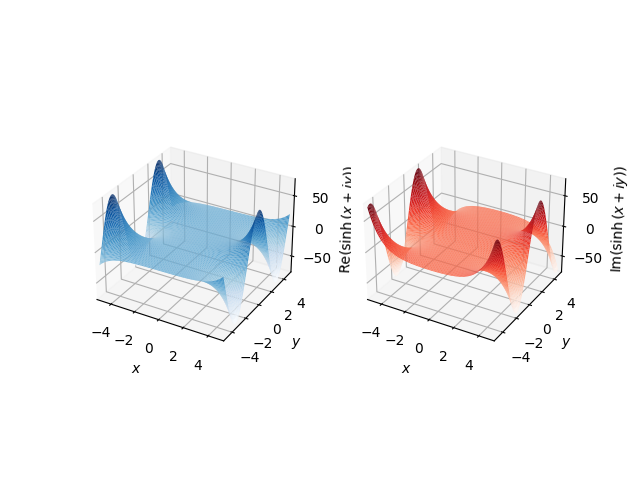
\includegraphics[width=0.8\textwidth]{figures/sinh_z.png}
	\caption{$\sinh(x+i y)$}
	\label{fig:sinh_z}
\end{figure}
\textbf{Properties of }$\sinh(z)$ 

\begin{enumerate}
	\item \textbf{Definition:}$\sinh z=\frac{1}{2}\left(e^z-e^{-z}\right)$
	\item \textbf{Domain/Range:} 
	\item \textbf{Derivative/Antiderivative:} The derivative is given by
\[
\frac{d}{d z} \sinh z=\cosh z,
\]
where $\cosh z$ is the hyperbolic cosine, and the indefinite integral by
\[
\int \sinh z d z=\cosh z+C,
\]
where $C$ is a constant of integration.
	\item \textbf{Branch cut:} 
	\item \textbf{Identities:}
\end{enumerate}

\begin{figure}[H]
	\centering
	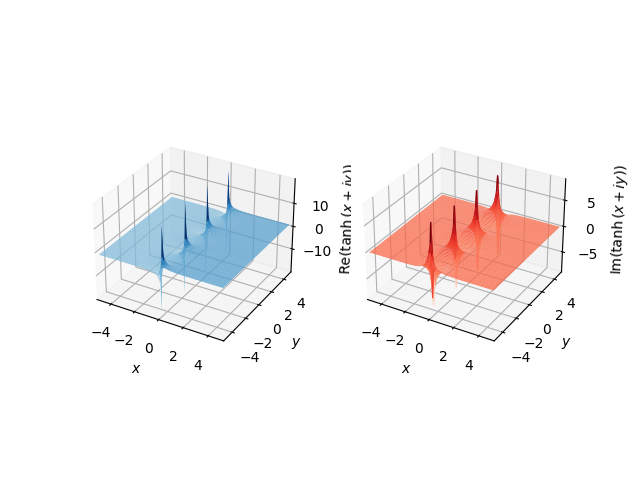
\includegraphics[width=0.8\textwidth]{figures/tanh_z.png}
	\caption{$\tanh(x+i y)$}
	\label{fig:tanh_z}
\end{figure}
\textbf{Properties of }$\tanh(z)$ 

\begin{enumerate}
	\item \textbf{Definition:} the hyperbolic tangent is defined as
\[
\begin{aligned}
\tanh z & \equiv \frac{\sinh z}{\cosh z} \\
&=\frac{e^z-e^{-z}}{e^z+e^{-z}} \\
&=\frac{e^{2 z}-1}{e^{2 z}+1}
\end{aligned}
\]
	\item \textbf{Domain/Range:} 
	\item \textbf{Derivative/Antiderivative:} 
		The derivative of $\tanh z$ is
		\[
			\frac{d}{d z} \tanh z=\operatorname{sech}^2 z
		\]

The indefinite integral is given by
\[
\int \tanh z d z=\ln (\cosh z)+C .
\]
	\item \textbf{Branch cut:} 
	\item \textbf{Identities:}
\end{enumerate}

